\section{Plot Generation}
Each block that is sent into the PlotGenerator is treated differently depending on what the block label is. 
There are four different block labels: 

\begin{itemize}
    \item[\textit{Empty: }] Block is converted into one plot with the label \textit{Empty}.
    \item[\textit{Building: }] Block is split into 1-2 plots with the label \textit{Manhattan}. The generated plots have the same area. An example can be seen in Figure \ref{fig:plot_split}. %Right now in master it's either skyscraper or Apartments, but in L-system-buildings it's only Manhattan. I'm going to write that's only manhattan-style buildings 
    \item[\textit{Park}/\textit{Parking: }] Block is converted into one plot with the label \textit{Park} or \textit{Parking} respectively.  
\end{itemize}

\begin{figure}[h!]
    \centering
  
    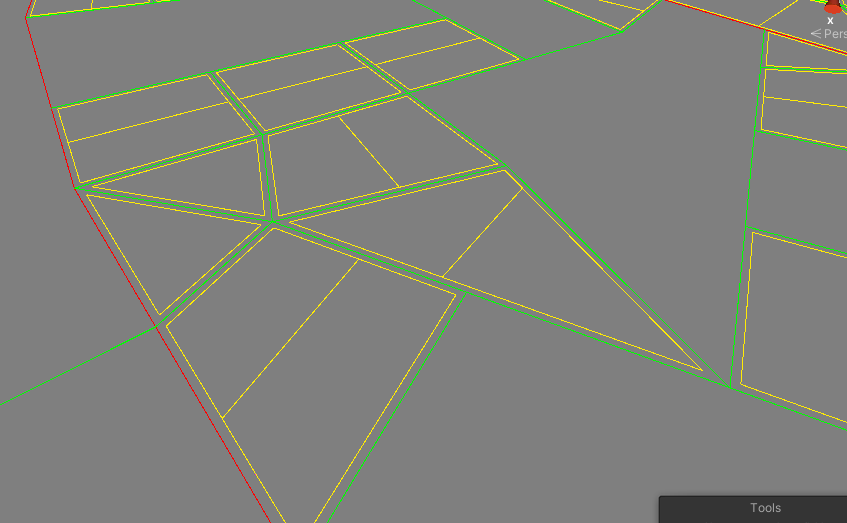
\includegraphics[width=0.8\textwidth]{figure/PlotSplit.png}
    \caption{Example of PlotGenerator splitting blocks with label \textit{Building}.}
  
    \label{fig:plot_split}
  \end{figure}
  
With the different plot labels, if not \textit{Empty}, respective generator are used to fill these plot of lands with content. 
